
% Spellcheck: ok
% Mikes: ok

\chapter{Models from Scaling Arguments}{}{}
\label{ch:scaling}

\index{data analysis!scaling|(}
\index{scaling|(}  

% Arguments from Scale

% ============================================================

\Fint{After familiarizing yourself with the data through plots and graphs,
the next step is to start} building a model for the data.  The meaning
of the word ``model'' is quite hazy, and I don't want to spend much
time and effort attempting to define this concept in an abstract way.
For our purposes, a \emph{model} is a mathematical description of the
data that ideally is guided by our understanding of the system under
consideration and that relates the various variables of the system to
each other: a ``formula.''

\section{Models}

\index{scaling!modeling principles|(}
\index{modeling!principles|(}  

Models like this are incredibly important. It is at this point that we
go from the merely \emph{descriptive} (plots and graphs) to the
\emph{prescriptive}: having a model allows us to predict what the
system will do under a certain set of conditions. Furthermore, a good
or truly useful model---because it helps us to \emph{understand} how
the system works---allows us to do so without resorting to the model
itself or having to evaluate any particular formula explicitly.  A
good model ties the different variables that control the system
together in such a way that we can see how varying any one of them
will influence the outcome. It is this use of models---as an aide to
or expression of our understanding---that is the most important one.
(Of course, we must still evaluate the model formulas explicitly in
order to obtain actual numbers for a specific prediction.)

I should point out that this view of models and what they can do is
not universal, and you will find the term used quite differently
elsewhere. For instance, statistical models (and this includes
machine-learning models) are much more descriptive: they do not
purport to \emph{explain} the observed behavior in the way just
described. Instead, their purpose is to predict expected outcomes\vadjust{\pagebreak} with
the greatest level of accuracy possible (numbers in, numbers out).  In
contrast, my training is in theoretical physics, where the development
of \emph{conceptual understanding} of the observed behavior is the
ultimate goal. I will use all available information about the system
and how it works (or how I \emph{suspect} it works!)  wherever I can;
I don't restrict myself to using only the information contained in the
data itself.  (This is a practice that statisticians traditionally
frown upon, because it constitutes a form of ``pollution'' of the
data. They may very well be right, but my purpose is different: I
don't want to understand the \emph{data}, I want to understand the
\emph{system}!) At the same time, I don't consider the absolute
accuracy of a model paramount: a model that yields only
order-of-magnitude accuracy but helps me understand the system's
behavior (so that I can, for instance, make informed trade-off
decisions) is much more valuable to me than a model that yields
results with 1 percent accuracy but that is a black box otherwise.

To be clear: there are situations when achieving the best possible
accuracy is all that matters and conceptual understanding is of little
interest. (Often these cases involve repeatable processes in
well-understood systems.) If this describes your situation, then you
need to use different methods that are appropriate to your problem
scenario.

% Statisticians will probably consider my models biased and inaccurate.
% I consider their models, basically, useless. 

\subsection{Modeling}

As should be clear from the preceding description, building models is
basically a creative process. As such, it is difficult (if not impossible)
to teach: there are no established techniques or processes for
arriving at a useful model in any given scenario. One common approach
to teaching this material is to present a large number of case
studies, describing the problem situations and attempts at modeling
them. I have not found this style to be very effective. First of all,
every (nontrivial) problem is different, and tricks and fortuitous
insights that work well for one example rarely carry over to a
different problem. Second, building effective models often requires
fairly deep insight into the particulars of the problem space, so you
may end up describing lots of tedious details of the \emph{problem}
when actually you wanted to talk about the \emph{model} (or the
modeling).

In this chapter, we will take a different approach.  Effective
modeling is often an exercise in determining ``what to leave out'':
good models should be simple (so that they are workable) yet retain
the essential features of the system---certainly those that we are
interested in.

As it turns out, there are a few essential arguments and approximations
that prove helpful again and again to make a complex problem tractable
and to identify the dominant behavior. That's what I want to talk about.

\index{scaling!modeling principles|)}
\index{modeling!principles|)}  

\subsection{Using and Misusing Models}

Just a reminder: models are not reality. They are descriptions or
approximations of reality---often quite coarse ones! We need to ensure
that we only place as much confidence in a model as is warranted.

How much confidence is warranted? That depends on how well- tested the
model is. If a model is based on a good theory, agrees well with a
wide range of data sets, and has shown it can predict observations
correctly, then our confidence may be quite strong.

At the other extreme are what one might call ``pie in the sky''
models: ad hoc models, involving half a dozen (or so) parameters---all
of which have been estimated independently and not verified against
real data. The reliability of such a model is highly dubious: each of
the parameters introduces a certain degree of uncertainty, which in
combination can make the results of the model meaningless. Recall the
discussion in Chapter \ref{ch:guesstimation}: three parameters known
to within 10 percent produce an uncertainty in the final result of 30
percent---and that assumes that the parameters are actually known to
within 10 percent! With four to six parameters that possibly are known,
only much less precisely than 10 percent, the situation is
correspondingly worse.  (Many business models fall into this
category.)

Also keep in mind that virtually all models have only a limited region
of validity. If you try to apply an existing model to a drastically
different situation or use input values that are very different from
those that you used to build the model, then you may well find that
the model makes poor predictions. Be sure to check that the
assumptions on which the model is based are actually fulfilled for
each application that you have in mind!


\vspace*{-6pt}
% ============================================================
\section{Arguments from Scale}

\index{scaling!arguments|(}
\index{arguments, scaling|(}
  
Next to the local stadium there is a large, open parking lot. During
game days, the parking lot is filled with cars, and---for obvious
reasons---a line of portable toilets is set up all along one of the
edges of the parking lot. This poses an interesting balancing problem:
will this particular arrangement work for all situations, no matter
how large the parking lot in question?

The answer is no. The number of people in the parking lot grows with
the area of the parking lot, which grows with the square of the edge
length (\ie, it ``scales as'' $L^2$); but the number of toilets is
proportional to the edge length itself (so it scales as $L$).
Therefore, as we make the parking lot bigger and bigger, there comes a
point where the number of people overwhelms the number of available
facilities. Guaranteed.

\vspace*{-6pt}
\subsection{Scaling Arguments}

This kind of reasoning is an example of a \emph{scaling argument}.
Scaling arguments try to capture how some quantity of interest depends
on a control parameter. In particular, a scaling argument describes
how the output quantity will change as the control parameter changes.
Scaling arguments are a particularly fruitful way to arrive at
symbolic expressions for phenomena (``formulas'') that can be
manipulated analytically.

You should have observed that the expressions I gave in the
introductory example were not ``dimensionally consistent.'' We had
people expressed\vadjust{\pagebreak} as the square of a length and toilets expressed as
length---what is going on here?  Nothing, I merely omitted some detail
that was not relevant for the argument I tried to make. A car takes up
some amount of space on a parking lot; hence given the size of the
parking lot (its area), we can figure out how many cars it can
accommodate.  Each car seats on average two people (on a game day), so
we can figure out the number of people as well. Each person has a
certain probability of using a bathroom during the duration of the
game and will spend a certain number of minutes there. Given all these
parameters, we can figure out the required ``toilet availability
minutes.'' We can make a similar argument to find the ``availability
minutes'' provided by the installed facilities. Observe that none of
these parameters depend on the size of the parking lot: they are
constants. Therefore, we don't need to worry about them if all we want
to determine is whether this particular arrangement (with toilets all
along one edge, but nowhere else) will work for parking lots of any
size. (It is a widely followed convention to use the \emph{tilde}, as
in $A \sim B$, to express that $A$ ``scales as'' $B$, where $A$ and
$B$ do not necessarily have the same dimensions.)

On the other hand, if we actually want to know the exact number of
toilets required for a specific parking lot size, then we do need to
worry about these factors and try to obtain the best possible
estimates for them.

Because scaling arguments free us from having to think about pesky
numerical factors, they provide such a convenient and powerful way to
begin the modeling process. At the beginning, when things are most
uncertain and our understanding of the system is least developed, they
free us from having to worry about low-level details (\eg, how long
does the average person spend in the bathroom?) and instead help us
concentrate on the system's overall behavior. Once the big picture has
become clearer (and if the model still seems worth pursuing), we may
want to derive some actual numbers from it as well. Only at this point
do we need to concern ourselves with numerical constants, which we
must either estimate or derive from available data.

A recurring challenge with scaling models is to find the correct
scales. For example, we implicitly assumed that the parking lot was
square (or at least nearly so) and would remain that shape as it grew.
But if the parking lot were growing in one direction only (\ie,
becoming longer and longer, while staying the same width), then its
area would no longer scale as $L^2$ but instead scale as $L$, where
$L$ is now the ``long'' side of the lot. This changes the argument, for
if the portable toilets were located along the long side of the lot
then the balance between people and available facilities would be the
same no matter how large the lot became! On the other hand, if the
facilities were set up along the short side, then their number would
remain constant while the long side grew, resulting again in an
imbalanced situation.

Finding the correct scales is a bit of an experience issue---the
important point here is that it is not as simple as saying: ``It's an
area, therefore it must scale as length squared.'' It depends on the
shape of the area and on which of its lengths controls the size.

% ``This whole business of scaling is a combination of experience
% and plain common sense.'' (Howison, Practical Applied Mathematics, p42)

The parking lot example demonstrates one typical application of
high-level scaling arguments: what I call a ``no-go argument.'' Even
without any specific numbers, the scaling behavior alone was enough to
determine that this particular arrangement of toilets to visitors will
break down at some point.

\subsection{Example: A Dimensional Argument}

\index{dimensional argument example!}
 
Figure \ref{fig:heightweight1} shows the heights and weights of a
class of female middle-school students.\footnote{A description of this
  data set can be found in \cit{A Handbook of Small Data Sets}{David
    J.\ Hand, Fergus Daly, K.\ McConway, D.\ Lunn, and E.
    Ostrowski}{Chapman \& Hall/CRC}{1993}}  Also displayed is the
function $m = 0.84 h - 84.0$, where $m$ stands for the mass (or
weight) and $h$ for the height. The fit seems to be quite close---is
this a good model?

\begin{figure}
  \centerline{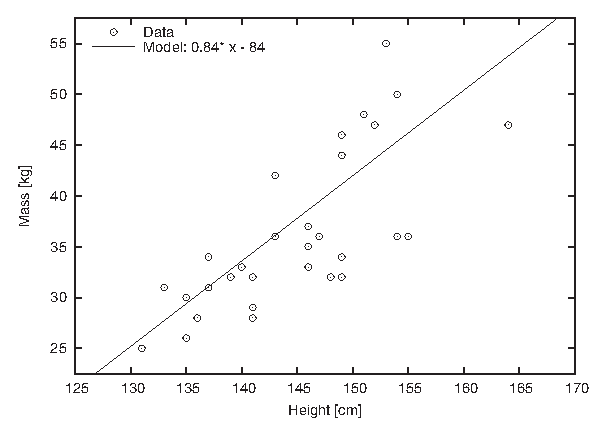
\includegraphics{img/heightweight1}}
  \caption{Heights and weights of a group of middle-school students.}
  \label{fig:heightweight1}
\end{figure}

The answer is no, because the model makes unreasonable predictions.
Look at it: the model suggests that students have no weight unless
they are at least $84$ centimeters (almost 3 feet) tall; if they were
shorter, their weight would be \emph{negative}. Clearly, this model is
no good (although it does \emph{describe} the data over the range
shown quite well). We expect that people  who have no height also have
no weight, and our model should reflect that.

Rather than a model of the form $a x + b$, we might instead try $a
x^b$, because this is the simplest function that gives the expected
result for $x=0$.

\begin{figure}
\centerline{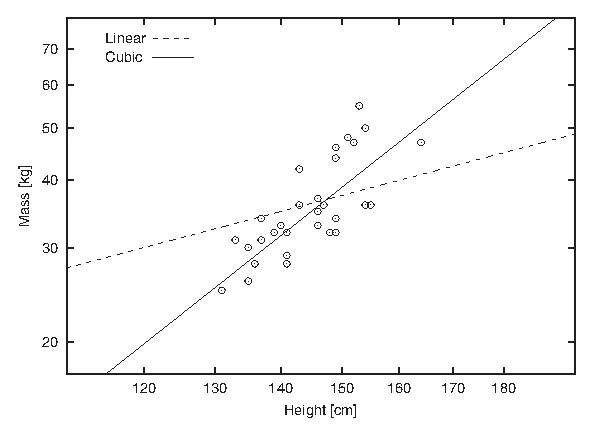
\includegraphics{img/heightweight2}}
  \caption{A double logarithmic plot of the data from Figure
    \ref{fig:heightweight1}.  The cubic function ${m} = {ah}^3$ seems to
    describe the data much better than the linear function ${m} = {ah}$.}
  \label{fig:heightweight2}
\end{figure}\pagebreak

Figure \ref{fig:heightweight2} shows the same data but on a double
logarithmic plot. Also indicated are functions of the form $y=a x$ and
$y=ax^3$. The cubic function $a x^3$ seems to represent the data quite
well---certainly better than the linear function.

But this makes utmost sense! The weight of a body is proportional to
its \emph{volume}---that is, to height times width times depth or $h
\cdot w \cdot d$.  Since body proportions are pretty much the same for
all humans (\ie, a person who is twice as tall as another will have
shoulders that are twice as wide, too), it follows that the volume of a
person's body (and hence its mass) scales as the third power of the
height: $\text{mass} \sim \text{height}^3$.

\begin{figure}
  \centerline{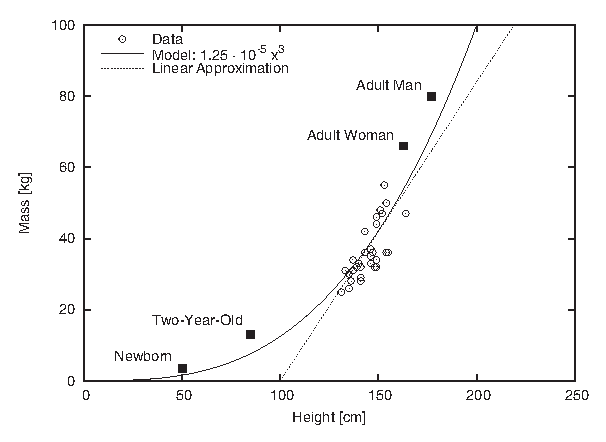
\includegraphics{img/heightweight3}}
  \caption{The data from Figure \ref{fig:heightweight1}, together with
    the cubic model and the linear approximation to this model around
    ${h}=\hbox{\em 150}\, { cm}$. Note that the approximation is good over the
    range of the actual data set but is wildly off farther away from
    it.}
  \label{fig:heightweight3}
\end{figure}

Figure \ref{fig:heightweight3} shows the data one more time and
together with the model $m = 1.25 \cdot 10^{-5} h^3$. Notice that the
model makes reasonable predictions even for values outside the range
of available data points, as you can see by comparing the model
predictions with the average body measurements for some different age
groups. (The figure also shows the possible limitations of a model
that is built using less than perfectly representative data: the model
underestimates adult weights because middle-school students are
relatively light for their size. In contrast, two-year-olds are
notoriously ``chubby.'')

Nevertheless, this is a very successful model. On the one hand,
although based on very little data, the model successfully predicts
the weight to within 20 percent accuracy over a range of almost two
orders of magnitude in height. On the other hand, and arguably more
importantly, it captures the general relationship between body height
and weight---a relationship that makes sense but that we might not
necessarily have guessed without looking at the data.

The last question you may ask is why the initial description, $m =
0.84 x - 84$ in Figure \ref{fig:heightweight1} seemed so good. The
answer is that this is exactly the linear approximation to the correct
model, $m = 1.25 \cdot 10^{-5} h^3$, near $h = 150 \text{ cm}$. (See
Appendix \ref{app:calculus}.)  As with all linear approximations, it
works well in a small region but fails for values farther away.

\subsection{Example: An Optimization Problem}

\index{optimization problems!scaling}
 
Another application of scaling arguments is to cast a question as an
optimization problem. Consider a group of people scheduled to perform
some task (say, a programming team). The amount of work that this
group can perform in a fixed amount of time (its ``throughput'') is
obviously proportional to the number $n$ of people on the team: $\sim
n$. However, the members of the team will have to coordinate with each
other. Let's assume that each member of the team needs to talk to
every other member of the team at least once a day.  This implies a
communication overhead that scales the \emph{square} of the number of
people: $\sim -n^2$. (The minus sign indicates that the communication
overhead results in a loss in throughput.) This argument alone is
enough to show that for this task, there is an optimal number of people
for which the realized productivity will be highest. (Also see Figure
\ref{fig:scalingopt}.)

\begin{figure}
\centerline{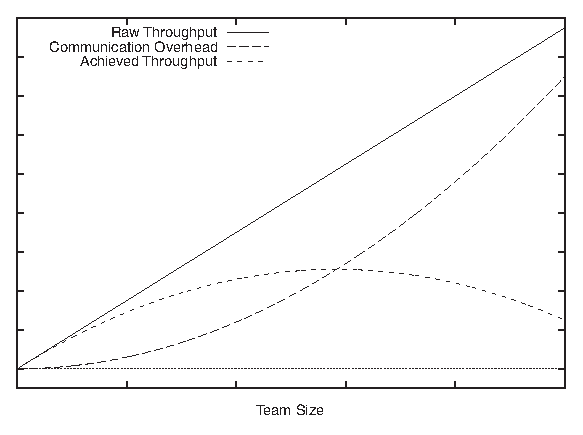
\includegraphics{img/scalingopt}}
  \caption{The work achievable by a team as a function of its size:
    the raw amount of work that can be accomplished grows with the
    team size, but the communication overhead grows even faster, which
    leads to an optimal team size.}
  \label{fig:scalingopt}\vspace*{-12pt}
\end{figure}

To find the optimal staffing level, we want to maximize the
productivity $P$ with respect to the number of workers on the team
$n$:
%
\[
P(n) = c n - d n^2
\]
%
where $c$ is the number of minutes each person can contribute during a
regular workday, and $d$ is the \emph{effective} number of minutes
consumed by each communication event. (I'll return to the cautious
``effective'' modifier shortly.)

To find the maximum, we take the derivative of $P(n)$ with respect to
$n$, set it equal to $0$, and solve for $n$ (see Appendix
\ref{app:calculus}).  The result is:
%
\[
n_{\text{\scriptsize optimal}} = \frac{c}{2d}
\]
%
Clearly, as the time consumed by each communication event $d$ grows
larger, the optimal team size shrinks.

If we now wish to find an actual number for the optimal staffing
level, then we need to worry about the numerical factors, and this is
where the ``effective'' comes in. The total number of hours each
person can put in during a regular workday is easy to estimate 
(8~hours at 60 minutes, less time for diversions), but the amount of
time spent in a single communication event is more difficult to
determine. There are also additional effects that I would lump into
the ``effective'' parameter: for example, not everybody on the team
needs to talk to everybody else. Adjustments like this can be lumped
into the parameter $d$ which increasingly turns it into a synthetic
parameter and less one that can be measured directly.

\subsection{Example: A Cost Model}
\index{costs!cost model example}
Models don't have to be particularly complicated to provide important
insights. I remember a situation where we were trying to improve the
operation of a manufacturing environment. One particular job was
performed\vadjust{\pagebreak} on a special machine that had to be retooled for each
different type of item to be produced. First the machine would be set
up (which took about 5 to 10 minutes), and then a worker would
operate the machine to produce a batch of 150 to 200 identical items.
The whole cycle lasted a bit longer than an hour and a half to
complete the batch, and then the machine was retooled for the next
batch.

The retooling part of the cycle was a constant source of management
frustration: for 10~minutes (while the machine was being set up),
nothing seemed to be happening. Wasted time! (In manufacturing,
productivity---defined as ``units per hour''---is the most closely
watched metric.)  Consequently, there had been a long string of
process improvement projects dedicated to making the retooling part
more efficient and thereby faster. By the time I arrived, it had been
streamlined very well. Nevertheless, there were constant efforts
underway to reduce the time it took---after all, the sight of the
machine sitting idle for 10~minutes seemed to be all the proof that
was needed.

It is interesting to set up a minimal cost model for this process.
The relevant quantity to study is ``minutes per unit.'' This is
essentially the inverse of the productivity, but I find it easier to
think in terms of the time it takes to produce a single unit than the
other way around. Also note that ``time per unit'' equates to ``cost
per unit'' after we take the hourly wage into account. Thus, the time
per unit is the time $T$ it takes to produce an entire batch, divided
by the number of items $n$ in the batch. The total processing time
itself consists of the setup time $T_1$ and $n$ times the amount of
time $t$ required to produce a single item:
%
\begin{align*}
\frac{T}{n} & = \frac{ T_1 + n t }{n} \\
            & = \frac{T_1}{n} + t
\end{align*}
%
The first term on the righthand side is the amount of the setup time
that can be attributed to a single item; the second term, of course,
is the time it takes to actually produce the item. The larger the
batch size, the smaller the contribution of the setup time to the cost
of each item as the setup time is ``amortized'' over more units.

\begin{figure}
  \centerline{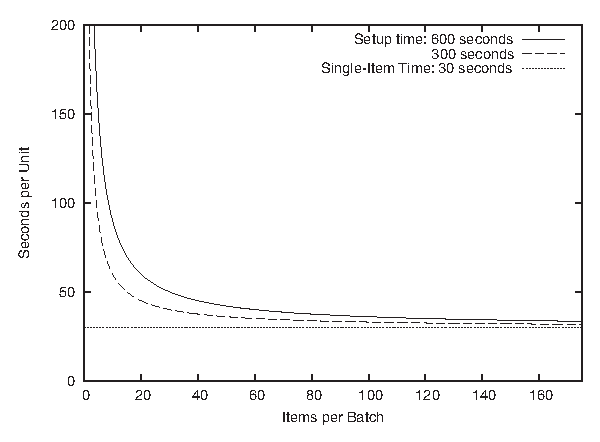
\includegraphics{img/batchsize}}
  \caption{Total time required to process a unit, as a function of the
    batch size.}
  \label{fig:batchsize}
\end{figure}

This is one of those situations where the numerical factors actually
matter. We know that $T_1$ is in the range of 300--600 seconds, and
that $n$ is between $150$ and $200$, so that the setup time per item,
$T_1/n$, is between 1--4 seconds. We can also find the time $t$ required
to actually produce a single item if we recall that the cycle time for
the entire batch was about $90$ minutes; therefore $t = 90 \cdot 60
/n$, which is about $30$ seconds per item. In other words, the setup
time that caused management so much grief actually accounted for less
than 10 percent of the total time to produce an item!

But we aren't finished yet. Let's assume that, through some strenuous
effort, we are able to reduce the setup time by 10 percent. (Not very
likely, given that this part of the process had already received a lot
of attention, but let's assume---best case!) This would mean that we
can reduce the setup time \emph{per item} to 1--3.5 seconds. However,
this means that the \emph{total} time per\vadjust{\pagebreak} item is reduced by only $1$
or $2$ percent! This is the kind of efficiency gain that makes sense
only in very, very controlled situations where \emph{everything} else
is completely optimized. In contrast, a $10$ percent reduction in $t$,
the actual work time per item, would result in (almost) a $10$ percent
improvement in overall productivity (because the amount of time that
it takes to produce an item is so much greater than the fraction of
the setup time attributable to a single item).

We can see this in Figure \ref{fig:batchsize} which shows the
``loaded'' time per unit (including the setup time) for two typical
values of the setup time as a function of the number of items produced
in a single batch.  Although the setup time contributes significantly
to the per-item time when there are fewer than about 50 items per
batch, its effect is very small for batch sizes of 150 or more. For
batches of this size, the time it takes to actually \emph{make} an
item dominates the time to retool the machine.

The story is still not finished. We eventually launched a project to
look at ways to reduce $t$ for a change, but it was never strongly
supported and shut down at the earliest possible moment by plant
management in favor of a project to look at, you guessed it, the setup
time! The sight of the machine sitting idle for 10~minutes was more
than any self-respecting plant manager could bear.

% The very important take-away message here is this: facts and numbers
% carry very little credibility, in the face of apparent (!) hands-on,
% immediate, visual evidence to the contrary. And in the face of
% long-standing habits.


% \subsection{Typical Scales and Collapsing Curves}
% \tbd

% collapsing curves (gaussians, pv=NRT, empirical?)

\subsection{Optional: Scaling Arguments Versus Dimensional Analysis}

\index{dimensional analysis versus scaling arguments}
 
Scaling arguments may seem similar to another concept you may have
heard of: \emph{dimensional analysis}. Although they are related, they
are really quite different. Scaling concepts, as introduced here, are
based on our intuition of how the system behaves and are a way to
capture this intuition in a mathematical expression.

Dimensional analysis, in contrast, applies to physical systems, which
are described by a number of quantities that have different physical
\emph{dimensions}, such as length, mass, time, or temperature. Because
equations describing a physical system must be dimensionally
consistent, we can try to deduce the form of these equations by forming
dimensionally consistent combinations of the relevant variables.

Let's look at an example. Everybody is familiar with the phenomenon of
air resistance, or drag: there is a force $F$ that acts to slow a
moving body down. It seems reasonable to assume that this force
depends on the cross-sectional area of the body $A$ and the speed 
(or velocity) $v$.
But it must also depend on some property of the medium (air, in this
case) through which the body moves. The most basic property is the
density $\rho$, which is the mass (in grams or kilograms) per volume
(in cubic centimeters or meters):
%
\[
F = f( A, v, \rho )
\]
%
Here, $f(x,y,z)$ is an as-yet-unknown function. 

Force has units of $\text{mass} \cdot \text{length}^2/\text{time}^2$,
area has units of $\text{length}^2$, velocity of
$\text{length}/\text{time}$, and density has units of
$\text{mass}/\text{length}^3$. We can now try to combine $A$, $v$, and
$\rho$ to form a combination that has the same dimensions as force. A
little experimentation leads us to:
%
\[
F = c \rho A v^2
\]
%
where $c$ is a pure (dimensionless) number. This equation expresses
the well-known result that air resistance increases with the square of
the speed. Note that we arrived at it using purely dimensional
arguments without any insight into the physical mechanisms at work.

This form of reasoning has a certain kind of magic to it: why did we
choose these specific quantities? Why did we not include the viscosity
of air, the ambient air pressure, the temperature, or the length of
the body? The answer is (mostly) physical intuition.  The viscosity
of air is small (viscosity measures the resistance to shear stress,
which is the force transmitted by a fluid captured between parallel
plates moving parallel to each other but in opposite
directions---clearly, not a large effect for air at macroscopic length
scales). The pressure enters indirectly through the density (at
constant temperature, according to the ideal gas law). And the length
of the body is hidden in the numerical factor $c$, which depends on
the shape of the body and therefore on the ratio of the
cross-sectional radius $\sqrt{A}$ to the length. In summary: it is
impressive how far we came using only very simple arguments, but it is
hard to overcome a certain level of discomfort entirely.

Methods of dimensional analysis appear less arbitrary when the
governing equations are known. If this is the case, then we can use
dimensional arguments to reduce the number of independently variable
quantities.  For example: \emph{assume} that we already know the drag
force is described by $F = c \rho A v^2$. Suppose  further that we want
to perform experiments to determine $c$ for various bodies by
measuring the drag force on them under various conditions. Naively, it
might appear\vadjust{\pagebreak} as if we had to map out the full three-dimensional
parameter space by making measurements for all combinations of $(\rho,
A, v)$. But these three parameters only occur in the combination
$\gamma = \rho A v^2$, therefore it is sufficient to run a single
series of tests that varies $\gamma$ over the range of values that we
are interested in. This constitutes a significant simplification!

Dimensional analysis relies on dimensional consistency and therefore
works best for physical and engineering systems, which are described
by independently measurable, dimensional quantities.  It is
particularly prevalent in areas such as fluid dynamics, where the
number of variables is especially high, and the physical laws are
complicated and often not well understood. It is much less applicable
in economic or social settings, where there are fewer (if any)
rigorously established, dimensionally consistent relationships.

\subsection{Other Arguments}

There are other arguments that can be useful when attempting to
formulate models. They come from the physical sciences, and (like
dimensional analysis) they may not work as well in social and economic
settings, which are not governed by strict physical laws.\vspace*{6pt}

\begin{unnumlist}
\subparagraph{Conservation laws}
\item Conservation \index{conservation laws} laws tell us that some quantity
  does not change over time. The best-known example is the law of
  conservation of energy. Conservation laws can be very powerful (in
  particular when they are exact, as opposed to only approximate) but
  may not be available: after all, the entire idea of economic growth
  and (up to a point) manufacturing itself rest on the assumption that
  more comes out than is being put in!\vspace*{6pt}

\subparagraph{Symmetries}
\item Symmetries, \index{symmetry!models} too, can be helpful in reducing
  complexity. For example, if an apparently two-dimensional system
  exhibits the symmetry of a circle, then I know that I'm dealing with
  a one-dimensional problem: any variation can occur only in the
  \emph{radial} direction, since a circle looks the same in all
  directions. When looking for symmetries, don't restrict yourself to
  geometric considerations---for instance, items entering and leaving
  a buffer at the same rate exhibit a form of symmetry. In this case,
  you might only need to solve one of the two processes explicitly
  while treating the other as a mirror image of the first.\vspace*{6pt}

\subparagraph{Extreme-value considerations}\index{extreme-value considerations}
\item How does the system behave at the
  extremes? If there are no customers, messages, orders, or items? If
  there are infinitely many? What if the items are extremely large or
  vanishingly small, or if we wait an infinite amount of time?  Such
  considerations can help to ``sanity check'' an existing model, but
  they can also provide inspiration when  first establishing a model.
  Limiting cases are often easier to treat because only one effect
  dominates, which eliminates the complexities arising out of the
  interplay of different factors.
\end{unnumlist}

% Little's law

\index{scaling!arguments|)}
\index{arguments, scaling|)}

% ============================================================
\section{Mean-Field Approximations}

\index{scaling!mean-field approximations|(}
\index{mean-field approximations|(}
 
The term \emph{mean-field approximation} comes from statistical
physics, but I use it only as a convenient and intuitive expression
for a much more general approximation scheme.

Statistical physics deals with large systems of interacting particles,
such as gas molecules in~a piston or atoms on a crystal lattice.
These systems are extraordinarily complicated because every particle
interacts with every other particle. If you move one of the particles,
then this will affect all the other particles, and so they will move,
too; but their movement will, in turn, influence the first
particle that we started with! Finding exact solutions for such large,
coupled systems is often impossible.  To make progress, we ignore the
individual interactions between explicit pairs of particles. Instead,
we assume that the~test particle experiences a field, the
``mean-field,'' that captures the ``average'' effect of all the other
particles.

For example, consider $N$ gas atoms in a bottle of volume $V$. We may
be interested to understand how often two gas atoms collide with each
other.  To calculate that number exactly, we would have to follow
every single atom over time to see whether it bumps into any of the
other atoms. This is obviously very difficult, and it certainly seems
as if we would need to keep track of a whole lot of detail that should
be unnecessary if we are only interested in macroscopic properties.

Realizing this, we can consider this gas in a mean-field
approximation: the probability that our test particle collides with
another particle should be proportional to the average density of
particles in that bottle $\rho = N/V$. Since there are $N$ particles
in the bottle, we expect that the number of collisions (over some time
frame) will be proportional to $N \rho$. This is good enough to start
making some predictions---for example, note that this expression is
proportional to $N^2$.  Doubling the number of particles in the bottle
therefore means that the number of collisions will grow by a factor of
$4$. In contrast, reducing the volume of the container by half will
increase the number of collisions only by a factor\break of $2$.

You will have noticed that in the previous argument, I omitted
lots of detail---for example, any reference to the time frame over
which I intend to count collisions. There is also a constant of
proportionality missing: $N \rho$ is not really the number of
collisions but is merely proportional to it. But if all I care about
is understanding how the number of collisions depends on the two
variables I consider explicitly (\ie, on $N$ and $V$), then I don't
need to worry about any of these details. The argument so far
is sufficient to work out how the number of collisions
scales with both $N$ and $V$. 

You can see how mean-field approximations and scaling arguments
enhance and support each other. Let's step back and look at the
concept behind mean-field approximations more closely.

\subsection{Background and Further Examples}

If mean-field approximations were limited to systems of interacting
particles, they would not be of much interest in this book. However,
the concept behind them is much more general and is very widely
applicable.

Whenever we want to calculate with a quantity whose values are
distributed according to some probability distribution, we face the
challenge that this quantity does not have a single, fixed value.
Instead, it has a whole spectrum of possible values, each more or less
likely according to the probability distribution. Operating with such
a quantity is difficult because at least in principle we have to
perform all calculations for each possible outcome and then weight the
result of our calculation by the appropriate probability. At the very
end of the calculation, we eventually form the average (properly
weighted according to the probability factors) to arrive at a unique
numerical value.

Given the combinatorial explosion of possible outcomes, attempting to
perform such a calculation exactly invariably starts to feel like
wading in a quagmire---and that assumes that the calculation can
be carried out exactly at all!

The mean-field approach cuts through this difficulty by performing the
average \emph{before} embarking on the actual calculation. Rather than
working with all possible outcomes (and averaging them at the end), we
determine the average outcome first and then only work with that value
alone. Table \ref{tbl:meanfield} summarizes the differences.

\begin{table}
\tabcolsep18pt
\def\vrl{\smash{\vrule height34pt width.25pt depth15pt}}
\tbl{Mean-field approximations replace an average over functions 
  with functions of averages.\label{tbl:meanfield}}{%
\begin{tabular}{ccc}\toprule
\TCH{Exact} & &\TCH{Mean-Field} \\\colrule
$E[x] = \sum\limits_{{\rm all\ outcomes}\ x} F(x) p(x)$ &\vrl&
$E_{{\rm MF}}[x] 
= F\paren{ \sum\limits_{{\rm all\ outcomes}\ x} x \, p(x) }$ 
\rule{0mm}{6mm} \\[12pt]
\end{tabular}}
\vspace*{-6pt}
\end{table}

This may sound formidable, but it is actually something we do all the
time.  Do you ever try to estimate how high the bill is going to be
when you are waiting in line at the supermarket? You can do this
explicitly---by going through all the items individually and adding up
their prices (approximately) in your head---or you can apply a
mean-field approximation by realizing that the items in your cart
represent a sample, drawn ``at random,'' from the selection of goods
available.  In the mean-field approximation, you would estimate the
average single-item price for goods from that store (probably about
\$5--\$7) and then multiply that value by the number of items in your
cart. Note that it should be much easier to count the items in your
cart than to add up their individual prices explicitly.

This example also highlights the potential pitfalls with mean-field
arguments: it will only be reliable if the average item price is a
good estimator. If your cart contains two bottles of champagne and a
rib roast for a party of eight, then an estimate based on a typical
item price of \$7 is going to be \emph{way} off.

To get a grip on the expected accuracy of a mean-field approximation,
we can try to find a measure for the width of the original
distribution (\eg, its standard deviation or inter-quartile range) and
then repeat our calculations after adding (and subtracting) the width
from the mean value. (We may also treat the width as a small
perturbation to the average value and use the perturbation methods
discussed in Chapter \ref{ch:guesstimation}.)

Another example: how many packages does UPS (or any comparable freight
carrier) fit onto a truck (to be clear: I don't mean a delivery
truck, but one of these 53 feet tractor-trailer long-hauls)? Well, we
can estimate the ``typical'' size of a package as about a cubic foot
($0.3^3 \text{ m}^3$), but it might also be as small as half that or
as large as twice that size. To find an estimate for the number of
packages that will fit, we divide the volume of the truck ($17$ m
long, $2$ m wide, $2.5$ m high---we can estimate height and width if
we realize that a person can stand upright in these things) by the typical
size of a package: $(17 \cdot 2 \cdot 2.5 / 0.3^3 ) \approx
\text{3,000}$ packages. Because the volume (not the length!) of each
package might vary by as much as a factor of $2$, we end up with lower
and upper bounds of (respectively) 1,500 to 6,000 packages.

This calculation makes use of the mean-field idea twice. First, we
work with the ``average'' package size. Second, we don't worry about
the actual spatial packing of boxes inside the truck; instead, we
pretend that we can reshape them like putty. (This also is a form of
``mean-field'' approximation.)

I hope you appreciate how the mean-field idea has turned this problem
from almost impossibly difficult to trivial---and I don't just mean
with regard to the actual computation and the eventual numerical
result; but more importantly in the way we thought about it.  Rather
than getting stuck in the enormous technical difficulties of working
out different stacking orders for packages of different sizes, the
mean-field notion reduced the problem description to the most
fundamental question: into how many small pieces can we divide a large
volume? (And if you think that all of this is rather trivial, I fully
agree with you---but the ``trivial'' can easily be overlooked when one
is presented with a complex problem in all of its ugly detail. Trying
to find mean-field descriptions helps strip away nonessential detail
and helps reveal the fundamental questions at stake.)

One common feature of mean-field solutions is that they frequently
violate some of the system's properties. For example, at Amazon, we
would often consider the typical order to contain $1.7$ items, of
which $0.9$ were books, $0.3$ were CDs, and the remaining $0.5$ items
were other stuff (or whatever the numbers were). This is obviously
nonsense, but don't let this disturb you!  Just carry on as if nothing
happened, and work out the correct breakdown of things at the end.
This approach doesn't always work: you'll still have to assign a whole
person to a job, even it requires only one tenth of a full-time
worker.  However, this kind of argument is often sufficient to work
out the general behavior of things.

There is a story involving Richard Feynman working on the Connection
Machine, one of the earliest massively parallel supercomputers.  All
the other people on the team were\vadjust{\pagebreak} computer scientists, and when a
certain problem came up, they tried to solve it using discrete methods
and exact enumerations---and got stuck with it. In contrast, Feynman
worked with quantities such as ``the average number of 1 bits in a
message address'' (clearly a mean-field approach). This allowed him to
cast the problem in terms of partial differential equations, which
were easier to solve.\footnote{This story is reported in
  \pcit{Richard Feynman and the Connection Machine}{Daniel
    Hillis}{Physics Today}{42}{February 1989}{78} The paper can also
  be found on the Web.}

\index{scaling!mean-field approximations|)}
\index{mean-field approximations|)}

% ============================================================
\section{Common Time-Evolution Scenarios}

\index{scaling!time-evolution scenarios|(}
\index{time-evolution scenarios|(}  

Sometimes we can propose a model based on the way the system under
consideration evolves. The ``proper'' way to do this is to write down
a differential equation that describes the system (in fact, this
is exactly what the term ``modeling'' often means) and then 
proceed to solve it, but that would take us too far afield.
(Differential equations relate the change in some quantity, expressed
through its derivative, to the quantity itself. These equations can be
solved to yield the quantity for all times.)

However, there are a few scenarios so fundamental and so common that
we can go ahead and simply write down the solution in its final form.
(I'll give a few notes on the derivation as well, but it's the
solutions to these differential equations that should be committed to
memory.)


\subsection{Unconstrained Growth and Decay Phenomena}

\index{time-evolution scenarios!unconstrained growth and decay phenomena}
\index{growth and decay phenomena, unconstrained}
  
The simplest case concerns pure growth (or death) processes. If the
\emph{rate} of change of some quantity is constant in time, then the
quantity will follow an \emph{exponential} growth (or decay). \index{exponential growth or decay} Consider
a cell culture. At every time step, a certain fraction of all cells in
existence at that time step will split (\ie, generate offspring).
Here the \emph{fraction} of cells that participate in the population
growth at every time step is constant in time; however, because the
population itself grows, the total number of new cells at each time
step is larger than at the previous time step. Many pure growth
processes exhibit this behavior---compound interest on a monetary
amount is another example (see Chapter \ref{ch:business}).

Pure death processes \index{death processes} work similarly, only in this case a constant
fraction of the population dies or disappears at each time step.
Radioactive decay is probably the best-known example; but another one
is the attenuation of light in a transparent medium (such as water).
For every unit of length that light penetrates into the medium, its
intensity is reduced by a constant fraction, which gives rise to the
same exponential behavior. In this case, the independent variable is
space, not time, but the argument is exactly the same.

Mathematically, we can express the behavior of a cell culture as
follows: if $N(t)$ is the number of cells alive at time $t$ and if
a fraction $f$ of these\vadjust{\pagebreak} cells split into new cells, then the number
of cells at the next time step $t+1$ will be:
%
\[
N(t+1) = N(t) + f N(t)
\]
%
The first term on the righthand side comes from the cells
which were already alive at time $t$, whereas the second term on
the right comes from the ``new'' cells created at $t$. We can now
rewrite this equation as follows:
%
\[
N(t+1) - N(t) = f N(t)
\]
%
This is a \emph{difference equation}. If we can assume that the time
``step'' is very small, we can replace the lefthand side with the
derivative of $N$ (this process is not always quite as simple as in
this example---you may want to check Appendix \ref{app:calculus} for
more details on difference and differential quotients): 
%
\[
\Diff{t}{N} = \frac{1}{T} N(t)
\]
\noindent This equation is true for growth processes; for pure death processes
instead we have an additional minus sign on the righthand side. 

These equations can be solved or integrated explicitly, and their
solutions are:
\begin{align*}
N(t) & = N_0 \, e^{t/T} \qquad & \text{Pure birth process\hskip3pt} \\
N(t) & = N_0 \, e^{-t/T}       & \text{ Pure death process} 
\end{align*}
Instead of using the ``fraction'' $f$ of new or dying cells that we
used in the difference equation, here we employ a characteristic
\emph{time scale} $T$, which is the time over which the number of
cells changes by a factor $e$ or $1/e$, where $e=2.71828\dots$.  The
value for this time scale will depend on the actual system: for cells
that multiply rapidly, $T$ will be smaller than for another species
that grows more slowly.  Notice that such a scale factor \emph{must}
be there to make the argument of the exponential function
dimensionally consistent!~Furthermore, the parameter $N_0$ is the
number of cells in existence at the beginning $t=0$.

Exponential processes (either birth or death) are very important, but
they never last very long. In a pure death process, the population
very quickly dwindles to practically nothing. At $t=3T$, only 5
percent of the original population are left; at $t=10T$, less than 1
in 10,000 of the original cells has survived; at $t=20T$, we are down
to one in a billion. In other words, after a time that is a small
multiple of $T$, the population will have all but disappeared.

Pure birth processes \index{birth processes} face the opposite problem: the population grows
so quickly that, after a very short while, it will exceed the capacity
of its environment. This is so generally true that it is worth
emphasizing: exponential growth is not sustainable over extended 
time periods. A process may start out as exponential, but before long,
it must and will saturate. That brings us to the next scenario.


\subsection{Constrained Growth: The Logistic Equation}

\index{time-evolution scenarios!constrained growth: the Logistic equation}
\index{growth, the logistic equation}
\index{logistic equations, constrained growth}
  
Pure birth processes never continue for very long: the population
quickly grows to a size that is unsustainable, and then the growth
slows. A common model that takes this behavior into account assumes
that the members of the population start to ``crowd'' each other,
possibly competing for some shared resource such as food or territory.
Mathematically, this can be expressed as follows:
%
\[
\Diff{t}{N} = \lambda N (K-N) \quad \text{$\lambda, K > 0$ fixed}
\]
%
The first term on the righthand side (which equals $\lambda K N$) is
the same as in the exponential growth equation. By itself, it would
lead to an exponentially growing population $N(t) = C \exp( \lambda K
t )$. But the second term ($- \lambda N^2$) counteracts this: it is
negative, so its effect is to \emph{reduce} the population; and it is
proportional to $N^2$, so it grows more strongly as $N$ becomes large.
(You can motivate the form of this term by observing that it measures
the number of collisions between members of the population and
therefore expresses the ``crowding'' effect.)

This equation is known as the \emph{logistic differential equation},
and its solution is the \emph{logistic function}:
%
\[
N(t) = \frac{K}{1 + \paren{ \frac{K}{N_0} -1 } e^{-\lambda K t} }
\]
%
This is a complicated function that depends on three parameters:
\begin{align*}
\lambda & \quad \text{The characteristic growth rate} \\
K       & \quad \text{The carrying capacity $K=N(t \to \infty)$} \\
N_0     & \quad \text{The initial number $N_0=N(t=0)$ of cells} 
\end{align*}
Compared to a pure (exponential) growth process, the appearance of the
parameter $K$ is new. It stands for the system's ``carrying
capacity''---that is the maximum number of cells that the environment
can support. \index{carrying capacity} You should convince yourself that the logistic function
indeed tends to $K$ as $t$ becomes large. (You will find different
forms of this function elsewhere and with different parameters,
but the form given here is the most useful one.) Figure
\ref{fig:logisticscaling} shows the logistic function for a selection
of parameter values.

\begin{figure}
\centerline{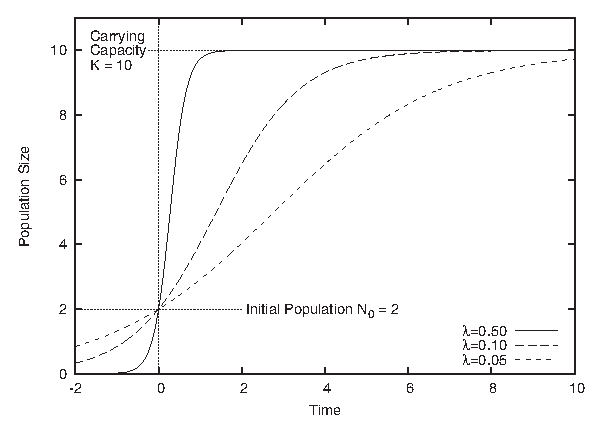
\includegraphics{img/logisticscaling}}
  \caption{Logistic growth for different values of the growth rate 
    $\lambda$. The initial population $N_0$ and the overall carrying
    capacity $K$ are the same in all cases.}
  \label{fig:logisticscaling}
\end{figure}

I should point out that determining values for the three parameters
from data can be extraordinarily difficult especially when the only
data points available are those to the left of the inflection point
(the point with maximum slope, about halfway between $N_0$ and $K$).
Many different combinations of $\lambda$, $K$, and $N_0$ may seem to
fit the data about equally well. In particular, it is difficult to
assess $K$ from early-stage data alone. You may want to try to obtain
an independent estimate (even a very rough one) for the carrying
capacity and use it when determining the remaining parameters from the
data.

The logistic function is the most common model for all growth
processes that exhibit some form of saturation. For example, infection
rates for contagious diseases can be modeled using the logistic
equation, as can the approach to equilibrium for cache hit rates.

\subsection{Oscillations}

\index{time-evolution scenarios!oscillations}
\index{oscillations, scaling} 
 
The last of the common dynamical behaviors occurs in systems in which
some quantity has an equilibrium value and that respond to excursions
from that equilibrium position with a restoring effect, which drives
the system back to the equilibrium position. If the system does not
come to rest in the equilibrium position but instead overshoots, then
the process will continue, going back and forth across the neutral
position---in other words, the system undergoes \emph{oscillation}.
Oscillations occur in many physical systems (from tides to grandfather
clocks to molecular bonds), but the ``restore and overshoot''
phenomenon is much more general. In fact, oscillations can be found
almost everywhere: the pendulum that has ``swung the other way'' is
proverbial, from the political scene to personal relationships.

Oscillations are periodic: the system undergoes the same motion again
and again. The simplest functions that exhibit this kind of behavior
are the trigonometric functions $\sin(x)$ and $\cos(x)$ (also see
Appendix \ref{app:calculus}), therefore we can express any periodic
behavior, at least approximately, in terms of sines or cosines. Sine
and cosine are periodic with period $2 \pi$. To express an oscillation
with period $D$, we therefore need to rescale $x$ by $2 \pi/D$. It may
also be necessary to shift $x$ by a phase factor $\phi$: an expression
like $\sin( 2 \pi (x-\phi)/D )$ will at least approximately describe
any periodic data set.

But it gets better: a powerful theorem states that \emph{every}
periodic function, no matter how crazy, can be written as a (possibly
infinite) combination of trigonometric functions called a
\emph{Fourier series}. \index{Fourier series} A Fourier series looks like this:
%
\[
f(x) = \sum_{n=1}^\infty a_n \sin\paren{2 \pi n \frac{x}{D}}
\]
%
where I have assumed that $\phi = 0$. The important point is that only
integer multiples of $2 \pi/D$ are being used in the argument of the
sine---the so-called ``higher harmonics'' of $\sin(2 \pi x/D)$.  We
need to adjust the coefficients $a_n$ to describe a data set.
Although the series is in principle infinite, we can usually get
reasonably good results by truncating it after only a few terms. (We
saw an example for this in Chapter \ref{ch:session}, where we used the
first two terms to describe the variation in $\mathrm{CO}_2$
concentration over Mauna Loa on Hawaii.)

\begin{figure}
\centerline{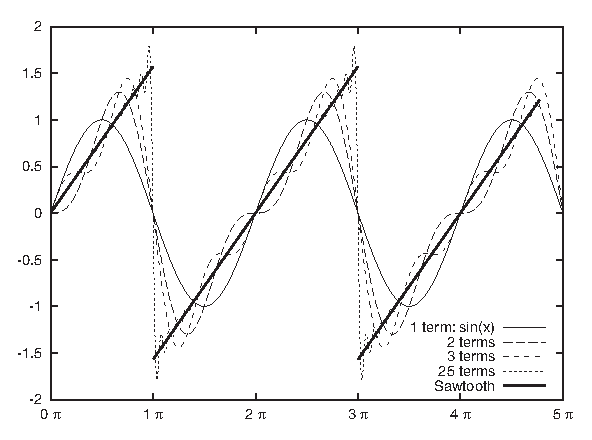
\includegraphics{img/fourier}}
  \caption{The sawtooth function can be composed out of sine functions
    and their higher harmonics.}
  \label{fig:fourier}
\end{figure}

If the function is known exactly, then the coefficients $a_n$ can be
worked out. For the sawtooth function (see Figure \ref{fig:fourier}),
the coefficients are simply $1, 1/2, 1/3, 1/4, \dots$ with alternating
signs:
%
\[
f(x) = \frac{\sin x}{1} - \frac{\sin 2x}{2} + \frac{\sin 3x}{3} \mp \dotsb
\]
%
You can see that the series converges quite rapidly---even for such a
crazy, discontinuous function as the sawtooth.

\index{scaling!time-evolution scenarios|)}
\index{time-evolution scenarios|)}  

% ============================================================
\section{Case Study: How Many Servers Are Best?}

\index{servers case study}
 
To close out this chapter, let's discuss an additional simple case
study in model building.

Imagine you are deciding how many servers to purchase to power your
ecommerce site. Each server costs you a fixed amount $E$ per
day---this includes both the operational cost for power and colocation
as well as the amortized acquisition cost (\ie, the purchase price
divided by the number of days until the server is obsolete and will be
replaced). The total cost for $n$ servers is therefore $n E$.

Given the expected traffic, one server should be sufficient to handle
the load.  However, each server has a finite probability $p$ of
failing on any given day. If your site goes down, you expect to lose
$B$ in profit before a new server can be provisioned and brought back
online.  Therefore, the expected loss when using a single server is $p
B$.

Of course, you can improve the reliability of your site by using
multiple servers.  If you have $n$ servers, then your site will be
down only if all of them fail simultaneously. The probability for this
event is $p^n$. (Note that $p^n < p$, since $p$ is a probability and
therefore $p < 1$.)

\begin{figure}
\centerline{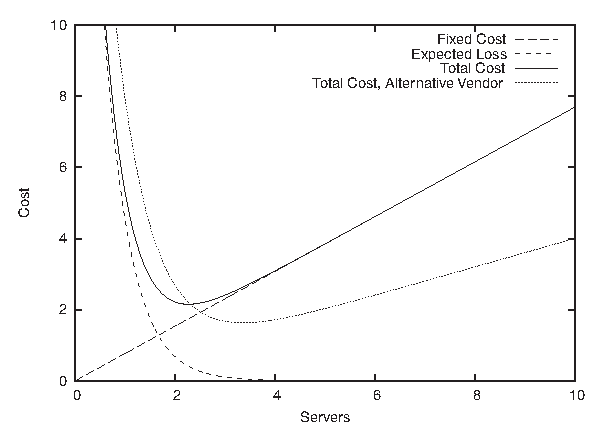
\includegraphics{img/serverdowntime}}
  \caption{Costs associated with provisioning a data center, as a 
    function of the number of servers.}
  \label{fig:serverdowntime}
\end{figure}

The total daily cost $C$ that you incur can now be written as the
combination of the fixed cost $n E$ and the expected loss due to
server downtime $p^n B$ (also see Figure \ref{fig:serverdowntime}):
%
\[
C = p^n B + n E
\]
%
Given $p$, $B$, and $E$, you would like to minimize this cost with
respect to the number of servers $n$. We can do this either analytically
(by taking the derivative of $C$ with respect to $n$) or numerically.

But wait, there's more! Suppose we also have an alternative proposal to
provision our data center with servers from a different\vadjust{\pagebreak} vendor. We
know that their reliability $q$ is worse (so that $q > p$), but their
price $F$ is significantly lower ($F \ll E$). How does this variant
compare to the previous one?

The answer depends on the values for $p$, $B$, and $E$. To make a
decision, we must evaluate not only the \emph{location} of the minimum
in the total cost (\ie, the number of servers required) but also the
actual \emph{value} of the total cost at the minimum position. Figure
\ref{fig:serverdowntime} includes the total cost for the alternative
proposal that uses less reliable but much cheaper servers. Although we
need more servers under this proposal, the total cost is nevertheless
lower than in the first one.

(We can go even further: how about a mix of different servers? This
scenario, too, we can model in a similar fashion and evaluate it 
against its alternatives.)


% ============================================================
\section{Why Modeling?}

\index{modeling!and data analysis} 

Why worry about modeling in a book on data \emph{analysis}?  It seems
we rarely have touched any actual data in the examples of this
chapter.

It all depends on your goals when working with data. If all you want
to do is to describe it, extract some features, or even decompose it
fully into its constituent parts, then the ``analytic'' methods of
graphical and data analysis will suffice. However, if you intend to
use the data to develop an understanding of the \emph{system} that
produced the data, then looking at the data itself will be only the
first (although important) step.

I consider conceptual modeling to be extremely important, because it
is here that we go from the descriptive to the prescriptive. A
conceptual model by itself may well be the most valuable outcome of an
analysis. But even if not, it will at the very least enhance the
purely analytical part of our work, because a conceptual model will
lead us to additional hypothesis and thereby suggest additional ways
to look at and study the data in an iterative process---in other
words, even a purely conceptual model will point us back to the data
but with added insight.

The methods described in this chapter and the next are the techniques
that I have found to be the most practically useful when thinking
about data and the processes that generated it. Whenever looking at
data, I always try to understand the system behind it, and I always
use some (if not all) of the methods from these two chapters.

% ============================================================
\section{Workshop: Sage}

\index{Sage|(} 

Most of the tools introduced in this book work with \emph{numbers},
which makes sense given that we are mostly interested in understanding
data. However, there is a different kind of tool that  works with
formulas instead: \emph{computer algebra systems}. The big
(commercial) brand names for such systems have been Maple and
Mathematica; in the open source world, the Sage project
(\url{http://www.sagemath.org}) has become somewhat of a front runner.

Sage is an ``umbrella'' project that attempts to combine several
existing open source projects (SymPy, Maxima, and others) together
with some added functionality into a single, coherent, Python-like
environment.\index{Python!Sage}\index{software!Python} Sage places heavy emphasis on features for number theory
and abstract algebra (not exactly everyone's cup of tea) and also
includes support for numerical calculations and graphics, but in this
section we will limit ourselves to basic calculus and a little linear
algebra.  (A word of warning: if you are not really comfortable with
calculus, then you probably want to skip the rest of this section.
Don't worry---it won't be needed in the rest of the book.)

Once you start Sage, it drops you into a text-based command
interpreter (a REPL, or read-eval-print loop). Sage makes it easy to
perform some simple calculations. For example, let's define a function
and take its derivative:
\begin{verbatim}
sage: a, x = var( 'a x' )
sage: f(x) = cos(a*x)
sage: diff( f, x )
x |--> -a*sin(a*x)
\end{verbatim}
In the first line we declare \texttt{a} and \texttt{x} as symbolic
variables---so that we can refer to them later and Sage knows how to
handle them. We then define a function using the ``mathematical''
notation \texttt{f(x) = \dots}. Only functions defined in this way can
be used in symbolic calculations. (It is also possible to define
Python functions using regular Python syntax, as in \texttt{def f(x,
  a): return cos(a*x)}, but such functions can only be evaluated
numerically.) Finally, we calculate the first derivative of the
function just defined.

All the standard calculus operations are available. We can combine
functions to obtain more complex ones, we can find integrals (both
definite and indefinite), and we can even evaluate limits:

\begin{verbatim}
sage: # Indefinite integral:
sage: integrate( f(x,a) + a*x^2, x )
1/3*a*x^3 + sin(a*x)/a
sage: 
sage: # Definite integral on [0,1]:
sage: integrate( f(x,a) + a*x^2, x, 0, 1 )
1/3*(a^2 + 3*sin(a))/a
sage: 
sage: # Definite integral on [0,pi], assigned to function:
sage: g(x,a) = integrate( f(x,a) + a*x^2, x, 0, pi )
sage: 
sage: # Evaluate g(x,a) for different a:
sage: g(x,1)
1/3*pi^3
sage: g(x,1/2)
1/6*pi^3 + 2
sage: g(x,0)
----------------------------------------------------------
RuntimeError

(some output omitted...)
\end{verbatim}
\begin{verbatim}

RuntimeError: power::eval(): division by zero
sage: limit( g(x,a), a=0 )
pi
\end{verbatim}

In the next-to-last command, we tried to evaluate an expression that
is mathematically not well defined: the function \texttt{g(x,a)}
includes a term of the form $\sin(\pi a)/a$, which we can't evaluate
for $a=0$ because we can't divide by zero. However, the limit $\lim_{a
  \to 0} \frac{\sin(\pi a)}{a} = \pi$ exists and is found by the
\texttt{limit()} function.

As a final example from calculus, let's evaluate some Taylor series
(the arguments are: the function to expand, the variable to expand in,
the point around which to expand, and the degree of the desired
expansion):

\begin{verbatim}
sage: taylor( f(x,a), x, 0, 5 )
1/24*a^4*x^4 - 1/2*a^2*x^2 + 1
sage: taylor( sqrt(1+x), x, 0, 3 )
1/16*x^3 - 1/8*x^2 + 1/2*x + 1
\end{verbatim}

So much for basic calculus. Let's also visit an example from linear
algebra. Suppose we have the linear system of equations:
%
\[
\begin{matrix}
a x & + & b y &   &     & = 1 \\
2 x & + & a y & + & 3 z & = 2 \\
b^2 x & &     & - &   z & = a 
\end{matrix}
\]
%
and that we would like to find those values of $(x, y, z)$ that solve
this system. If all the coefficients were numbers, then we could use a
numeric routine to obtain the solution; but in this case, some
coefficients are known only symbolically (as $a$ and $b$), and we would
like to express the solution in terms of these variables.

Sage can do this for us quite easily:

\begin{verbatim}
sage: a, b, x, y, z = var( 'a b x y z' )
sage: 
sage: eq1 = a*x + b*y == 1
sage: eq2 = 2*x + a*y + 3*z == 2
sage: eq3 = b^2 - z == a
sage: 
\end{verbatim}
\begin{verbatim}
sage: solve( [eq1,eq2,eq3], x,y,z )
[[x == (3*b^3 - (3*a + 2)*b + a)/(a^2 - 2*b), 
  y == -(3*a*b^2 - 3*a^2 - 2*a + 2)/(a^2 - 2*b), 
  z == b^2 - a]]
\end{verbatim}

As a last example, let's demonstrate how to calculate the eigenvalues
of the following matrix:
%
\[
M = 
\begin{pmatrix}
a & b & a \\
b & c & b \\
a & b & 0
\end{pmatrix}
\]
% 
Again, if the matrix were given numerically, then we could use a
numeric algorithm, but here we would like to obtain a symbolic
solution.

Again, Sage can do this easily:

\begin{verbatim}
sage: m = matrix( [[a,b,a],[b,c,b],[a,b,0]] )
sage: m.eigenvalues()
[-1/18*(-I*sqrt(3) + 1)*(4*a^2 - a*c + 6*b^2 + c^2)/(11/54*a^3 - 7/18*a^2*c + 1/3
*b^2*c + 1/27*c^3 + 1/18*(15*b^2 - c^2)*a + 1/18*sqrt(-5*a^6 - 6*a^4*b^2 + 11*a^2
*b^4 - 5*a^2*c^4 - 32*b^6 + 2*(5*a^3 + 4*a*b^2)*c^3 + (5*a^4 - 62*a^2*b^2 - 4*b^4
)*c^2 - 2*(5*a^5 + 17*a^3*b^2 - 38*a*b^4)*c)*sqrt(3))^(1/3) - 1/2*(I*sqrt(3) + 1)
*(11/54*a^3 - 7/18*a^2*c + 1/3*b^2*c + 1/27*c^3 + 1/18*(15*b^2 - c^2)*a + 1/18*sq
rt(-5*a^6 - 6*a^4*b^2 + 11*a^2*b^4 - 5*a^2*c^4 - 32*b^6 + 2*(5*a^3 + 4*a*b^2)*c^3
 + (5*a^4 - 62*a^2*b^2 - 4*b^4)*c^2 - 2*(5*a^5 + 17*a^3*b^2 - 38*a*b^4)*c)*sqrt(3
))^(1/3) + 1/3*a + 1/3*c, -1/18*(I*sqrt(3) + 1)*(4*a^2 - a*c + 6*b^2 + c^2)/(11/5
4*a^3 - 7/18*a^2*c + 1/3*b^2*c + 1/27*c^3 + 1/18*(15*b^2 - c^2)*a + 1/18*sqrt(-5*
a^6 - 6*a^4*b^2 + 11*a^2*b^4 - 5*a^2*c^4 - 32*b^6 + 2*(5*a^3 + 4*a*b^2)*c^3 + (5*
a^4 - 62*a^2*b^2 - 4*b^4)*c^2 - 2*(5*a^5 + 17*a^3*b^2 - 38*a*b^4)*c)*sqrt(3))^(1/
3) - 1/2*(-I*sqrt(3) + 1)*(11/54*a^3 - 7/18*a^2*c + 1/3*b^2*c + 1/27*c^3 + 1/18*(
15*b^2 - c^2)*a + 1/18*sqrt(-5*a^6 - 6*a^4*b^2 + 11*a^2*b^4 - 5*a^2*c^4 - 32*b^6 
+ 2*(5*a^3 + 4*a*b^2)*c^3 + (5*a^4 - 62*a^2*b^2 - 4*b^4)*c^2 - 2*(5*a^5 + 17*a^3*
b^2 - 38*a*b^4)*c)*sqrt(3))^(1/3) + 1/3*a + 1/3*c, 1/3*a + 1/3*c + 1/9*(4*a^2 - a
*c + 6*b^2 + c^2)/(11/54*a^3 - 7/18*a^2*c + 1/3*b^2*c + 1/27*c^3 + 1/18*(15*b^2 -
 c^2)*a + 1/18*sqrt(-5*a^6 - 6*a^4*b^2 + 11*a^2*b^4 - 5*a^2*c^4 - 32*b^6 + 2*(5*a
^3 + 4*a*b^2)*c^3 + (5*a^4 - 62*a^2*b^2 - 4*b^4)*c^2 - 2*(5*a^5 + 17*a^3*b^2 - 38
*a*b^4)*c)*sqrt(3))^(1/3) + (11/54*a^3 - 7/18*a^2*c + 1/3*b^2*c + 1/27*c^3 + 1/18
*(15*b^2 - c^2)*a + 1/18*sqrt(-5*a^6 - 6*a^4*b^2 + 11*a^2*b^4 - 5*a^2*c^4 - 32*b^
6 + 2*(5*a^3 + 4*a*b^2)*c^3 + (5*a^4 - 62*a^2*b^2 - 4*b^4)*c^2 - 2*(5*a^5 + 17*a^
3*b^2 - 38*a*b^4)*c)*sqrt(3))^(1/3)]
\end{verbatim}

Whether these results are useful to us is a different question!

This last example demonstrates something I have found to be quite
generally true when working with computer algebra systems: it can be
difficult to find the right kind of problem for them. Initially,
computer algebra systems seem like pure magic, so effortlessly do they
perform tasks that took us \emph{years} to learn (and that we still
get wrong). But as we move from trivial to more realistic problems, it
is often difficult to obtain results that are actually useful. All too
often we end up with a result like the one in the eigenvalue
example, which---although ``correct''---simply does not shed much
light on the problem we tried to solve!  And before we try manually to
simplify an expression like the one for the eigenvalues, we might be
better off solving the entire problem with paper and pencil, because
using paper and pencil, we can can introduce new variables for
frequently occurring terms or even make useful approximations as we
go along.

I think computer algebra systems are most useful in scenarios that
require the generation of a \emph{very} large number of terms (\eg,
combinatorial problems), which in the end are evaluated (numerically
or otherwise) entirely by the computer to yield the final result
without providing a ``symbolic'' solution in the classical sense at
all. When these conditions are fulfilled, computer algebra systems
enable you to tackle problems that would simply not be feasible with
paper and pencil. At the same time, you can maintain a greater level
of accuracy because numerical (finite-precision) methods, although
still required to obtain a useful result, are employed only in the
final stages of the calculation (rather than from the outset).\vadjust{\pagebreak} Neither
of these conditions is fulfilled for relatively straightforward ad hoc
symbolic manipulations. Despite their immediate ``magic'' appeal,
computer algebra systems are most useful as specialized tools for
specialized tasks!
One final word about the Sage project.  As an open source project, it
leaves a strange impression. You first become aware of this when you
attempt to download the binary distribution: it consists of a 500 MB
bundle, which unpacks to 2 GB on your disk! When you investigate what
is contained in this huge package, the answer turns out to be
\emph{everything}. Sage ships with \emph{all} of its dependencies. It
ships with its own copy of all libraries it requires. It ships with
its own copy of R. It ships with its own copy of Python!  In short, it
ships with its own copy of \emph{everything}.

This bundling is partially due to the well-known difficulties with
making deeply numerical software portable, but is also an expression
of the fact that Sage is an umbrella project that tries to combine a
wide range of otherwise independent projects. Although I sincerely
appreciate the straightforward pragmatism of this solution, it also
feels heavy-handed and ultimately unsustainable.  Personally, it makes
me doubt the wisdom of the entire ``all under one roof'' approach that
is the whole purpose of Sage: if this is what it takes, then we are
probably on the wrong track. In other words, if it is not feasible to
integrate different projects in a more organic way, then perhaps those
projects should remain independent, with the user free to choose which
to use.

% (It might be
% worth mentioning in this context that there are reports of hostile
% forks of projects who do not agree to being incorporated by Sage in
% this way.)

\index{Sage|)} 

% ============================================================
\section{Further Reading}

There are two or three dozen books out there specifically on the 
topic of modeling, but I have been disappointed by most of them.
Some of the more useful (from the elementary to the quite advanced)
include the following.

\begin{itemize}
\item \cit{How to Model It: Problem Solving for the Computer Age}{A.~M.\ Starfield, K.\ A.\ Smith, and A.~L.\ Bleloch}{Interaction Book
    Company}{1994}
  Probably the best elementary introduction to modeling that I am
  aware of. Ten (ficticious) case studies are presented and discussed,
  each demonstrating a different modeling method. (Out of print, but
  available used.)

%\item \cit{How to Model It: Problem Solving for the Computer Age}{A.\
%    M.\ Starfield, et al}{Interaction Book
%    Company}{1994}
%  Probably the best elementary introduction to modeling that I am
%  aware of. Ten (fictitious) case studies are presented and discussed,
%  each demonstrating a different modeling method. (Out of print but
%  available used.)

\item \cit{An Introduction to Mathematical Modeling}{Edward A.\
    Bender}{Dover Publications}{2000} 
  Short and idiosyncratic. A bit dated but still insightful.

\item \cit{Concepts of Mathematical Modeling}{Walter J.\ Meyer}{Dover
  Publications}{2004}
  This book is a general introduction to many of the topics required
  for mathematical modeling at an advanced beginner level. It feels
  more dated than it is, and the presentation is a bit pedestrian;
  % (some of the editorial comments in particular are not very insightful)
  nevertheless, it contains a lot of accessible, and most of all
  practical, material.

\item \cit{Introduction to the Foundations of Applied Mathematics}{Mark 
  H.\ Holmes}{Springer}{2009}
  This is one of the few books on modeling that places recurring 
  mathematical techniques, rather than case studies, at the center of its
  discussion. Much of the material is advanced, but the first\vadjust{\pagebreak} few chapters 
  contain a careful discussion of dimensional analysis and nice 
  introductions to perturbation expansions and time-evolution scenarios.

% \item \cit{...}{Mesterton-Gibbons}{...}{...}  
%   This is a rather thick book. Several examples and case studies are
%   analyzed throughout, using different methods and levels of
%   sophistication each time.  There is a lot of material here, but the
%   big picture is frequently lost among the wealth of (often
%   interesting) detail. Intermediate level.

\item \cit{Modeling Complex Systems}{Nino Boccara}{2nd ed., Springer}{2010}  
  This is a book by a physicist (not a mathematician, applied or
  otherwise), and it demonstrates how a physicist thinks about
  building models. The examples are rich, but mostly of theoretical
  interest. Conceptually advanced, mathematically not too difficult.
%  (A second edition is expected in late 2010.)

\item \cit{Practical Applied Mathematics}{Sam Howison}{Cambridge
    University Press}{2005}
  This is a very advanced book on applied mathematics with a 
  heavy emphasis on partial differential equations. However, the 
  introductory chapters, though short, provide one of the most
  insightful (and witty) discussions of models, modeling, scaling
  arguments, and related topics that I have seen.
\end{itemize}

The following two books are not about the process of modeling.
Instead, they provide examples of modeling in action (with a 
particular emphasis on scaling arguments):
\begin{itemize}
\item \cit{The Simple Science of Flight}{Henk Tennekes}{2nd ed., MIT
    Press}{2009}
  This is a short yet fascinating book about the physics and
  engineering of flying, written at the ``popular science'' level. The
  author makes heavy use of scaling laws throughout. If you are
  interested in aviation, then you will be interested in this book.

\item \cit{Scaling Concepts in Polymer Physics}{Pierre-Gilles de 
    Gennes}{Cornell University Press}{1979}
  This is a research monograph on polymer physics and probably not
  suitable for a general audience. But the treatment, which relies
  almost exclusively on a variety of scaling arguments, is almost
  elementary. Written by the master of the scaling models.
\end{itemize}
\index{data analysis!scaling|)} 
\index{scaling|)} 
\clearpage

\thispagestyle{empty}

\cleardoublepage